\section{Aufgabe 2.2: Dynamisches Erweitern von HTML-Dokumenten}
\begin{frame}[<+->]{Aufgabe 2.2}
\begin{center}
\normalsize{
Dynamisches Erweitern einer HTML- Datei mit DOM}
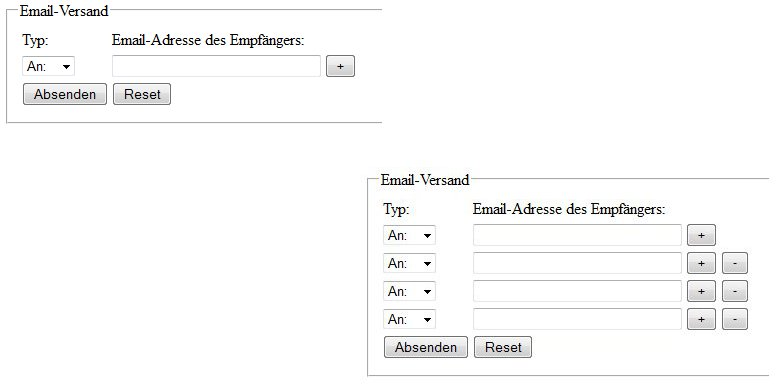
\includegraphics[width = 300px]{../A2/src/formular1.jpg}
\end{center}
\end{frame}
\tiny{\begin{lstlisting}[language = HTML,
                                   mathescape = true, 
                   breaklines=true, 
                   numbers = left,
	        firstnumber= 56, 
                   numbersep = 3pt]
<form onSubmit="return absenden(this)">
  <fieldset> <legend> Email-Versand </legend>
    <table border="0" cellpadding="0" cellspacing="4">
      <thead>
        <tr>
          <td>Typ:</td>
          <td>Email-Adresse des Empfaengers:</td>
        </tr>
      </thead>
      <tbody>
        <tr id="tr">
          <td> <select>
            <option>An:</option>
            <option>Cc:</option>
            <option>Bcc:</option>
          </select> </td>
          <td> <input type="text" size="30" maxlength="30"> </td>
          <td> <input type="button" value="+" onclick="zeile_neu()"> </td>
          <td> <input type="button" value="-" onclick="zeile_loeschen(this.parentNode)" style="visibility:hidden"> </td>
        </tr>
      </tbody>
      <tfoot>
        <tr>
          <td> <input type="submit" value="Absenden"> </td>
          <td> <input type="reset" value="Reset"> </td>
        </tr>
      </tfoot>
    </table>
  </fieldset>
</form>
\end{lstlisting}}
\begin{frame}[<+->][fragile]
\tiny{ \begin{lstlisting}[language = HTML,
                                   mathescape = true, 
                   breaklines=true, 
                   numbers = left,
	        firstnumber=66 , 
                   numbersep = 3pt]
<tr id="tr">
  <td><select>
     <option>An:</option>
     <option>Cc:</option>
     <option>Bcc:</option>
  </select></td>
  <td><input type="text" size="30" maxlength="30"></td>
  <td><input type="button" value="+" onclick="zeile_neu()"></td>
  <td><input type="button" value="-" onclick="zeile_loeschen(this.parentNode)" 
             style="visibility: hidden"></td>
</tr>
\end{lstlisting}}
\tiny{ \begin{lstlisting}[language=JavaScript, 
		   numbers=left,
		   numbersep=3pt,
		   firstnumber= 8,
		   breaklines=true]
function zeile_neu(){
	var Zeile = document.getElementById("tr");
	var Zeile_neu = Zeile.cloneNode(true);
	Zeile.parentNode.appendChild(Zeile_neu);
	Zeile_neu.getElementsByTagName("input")[2].style.visibility="visible";}
\end{lstlisting}}
\normalsize{
\begin{itemize}
\item Die Funktion zeile\_neu erzeugt dynamisch eine neue Formularzeile und macht in dieser den "-" Button sichtbar.
\end{itemize}
}
\end{frame}
\begin{frame}[<+->][fragile]
\tiny{ \begin{lstlisting}[language=JavaScript, 
		   numbers=left,
		   numbersep=3pt,
		   firstnumber= 8,
		   breaklines=true]
function zeile_loeschen(td){
  if(confirm("Sind sie wirklich sicher ?")==true){
    killElement(td.parentNode);
  }
}

function killElement(element){
  if (element) {
    var papa = element.parentNode;
    if (papa) papa.removeChild(element);
  }
}

\end{lstlisting}}
\tiny{ \begin{lstlisting}[language = HTML,
                                   mathescape = true, 
                   breaklines=true,  
                   numbersep = 3pt]
<td> <input type="button" value="-" onclick="zeile_loeschen(this.parentNode)" style="visibility:visible"> </td>
\end{lstlisting}}
\normalsize
\begin{itemize}
\item Die Funktion zeile\_loeschen loescht den Knoten, der die jeweilige Zeile repraesentiert. (siehe naechste Folie) 
\end{itemize}
\end{frame}
\begin{frame}[<+->]
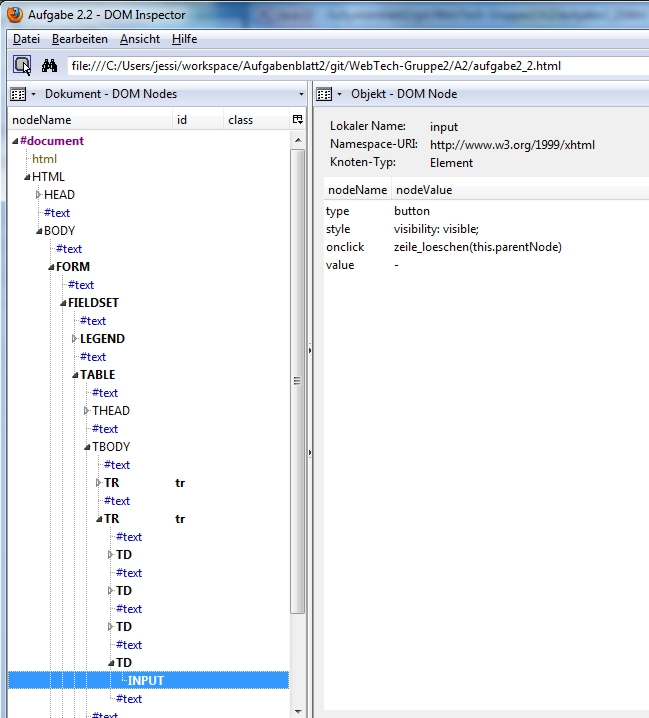
\includegraphics[width = 200px]{../A2/src/dom_inspector.jpg}
\end{frame}
\begin{frame}[<+->][fragile]
\tiny{\begin{lstlisting}[language=JavaScript, 
		   numbers=left,
		   numbersep=3pt,
		   firstnumber=28]
function absenden(form){
  var ausgabe="Empfaenger: \n";
  for(var i=1;i<form.elements.length;i++){
    if(form.elements[i].type == "button"){ }
    else if(form.elements[i].type == "reset"){ }
    else if(form.elements[i].type=="submit"){ }
    else if(form.elements[i].type=="text"){
      ausgabe = ausgabe + form.elements[i].value+" \n";
    }
    else{
      if(form.elements[i].selectedIndex == 0) {
        ausgabe = ausgabe + "An: ";	 
      }
      else if(form.elements[i].selectedIndex == 1) {
        ausgabe = ausgabe + "Cc: ";
      }
      else {
        ausgabe = ausgabe + "Bcc: "
      }
    }
  }
  alert(ausgabe);
}
\end{lstlisting}}
\tiny{\begin{lstlisting}[language = HTML,
                                   mathescape = true, 
                   breaklines=true,  
                   numbersep = 3pt]
<form onSubmit="absenden(this)">
\end{lstlisting}}
\normalsize
\begin{itemize}

\item Die Funktion absenden(this) sendet die Daten bei Drücken des Absenden-Button (type="submit") ab.

\end{itemize}
\end{frame}